\documentclass[fullscreen=true, unicode, bookmarks=false]{beamer}
\usepackage[T2A]{fontenc}
\usepackage[utf8]{inputenc}
\usepackage[english, russian]{babel}
\usepackage{amsmath}
\usepackage{amsmath,amsfonts,amssymb}
\usepackage[export]{adjustbox}
\usepackage{textgreek}
\newtheorem{rustheorem}{Утверждение }
\sloppy

\setbeamertemplate{navigation symbols}{}

\usetheme{Madrid}

\usecolortheme{whale}

\usefonttheme{professionalfonts} % default family is serif

\setbeamertemplate{footline}{\hspace*{.5cm}\scriptsize{\insertshorttitle
\hspace*{50pt} \hfill\hspace*{.5cm}}\vspace{5pt}} 

\setbeamercolor{bibliography entry author}{fg=black}

\title[]{ {\huge Бифуркационные особенности линейной краевой задачи с кубическим отклонением в краевом условии } } 
\date{ }  

\begin{document}

\begin{frame}
\titlepage
\end{frame} 

\begin{frame}
\frametitle{ Краевая задача с кубическим отклонением в краевом условии }
 
\begin{equation}
	\dot u = u'' + \gamma u,	
\end{equation}

\begin{equation}
	u'(0, t) \, = 0, \qquad u'(1, t) \, = \alpha\,u(x_0, t) + \beta u^3(x_0, t),
\end{equation}

\bigskip

$$ t \geqslant 0, \quad x \in [0,1]. $$


$$ \alpha, \gamma \in \mathbb{R}, \quad \beta \in \mathbb{R}\setminus\{ 0\}, \quad x_0 \in [0, 1). $$

\end{frame}

\begin{frame}
\frametitle{ Линеаризованная краевая задача }
 
\begin{equation}
	\dot u = u'' + \gamma u,	
\end{equation}

\begin{equation}	
	u'(0, t) \, = 0, \qquad u'(1, t) \, = \alpha_{cr}\,u(x_0, t).
\end{equation}

\end{frame}

\begin{frame}
\frametitle{ Задача на собственные значения }
 
$$ u(x, t) = e^{\lambda t} \, v(x). $$

\bigskip
 
\begin{equation}
	v'' + (\gamma - \lambda)v = 0,	
\end{equation}

\begin{equation}	
	v'(0) \, = 0, \qquad v'(1) \, = \alpha_{cr}\,v(x_0).
\end{equation}

\bigskip

$$ \mu = \sqrt{-\gamma + \lambda}, $$

$$ v(x) = c \ch  \mu x, \quad c \in \mathbb{R}. $$

\end{frame}

\begin{frame}
\frametitle{ Потеря устойчивости нулевого состояния равновесия }
 
\begin{equation}
	\mu \, \sh \mu \, = \, \alpha \ch \mu x_0,
\end{equation}

\medskip

\begin{itemize}

\item { $ \lambda = 0: \; \mu = \sqrt{-\gamma}, $ 
}

\begin{equation}
	\alpha_u = \frac{ \sqrt{-\gamma} \, \sh \sqrt{-\gamma} }{ \ch \sqrt{-\gamma} x_0 }.
\end{equation}

\item { $ \lambda = \pm i \omega: \; \mu = \sqrt{-\gamma + i \omega}, $ 
}

\begin{equation}
	\alpha_c = \frac{ \sqrt{-\gamma + i \omega} \, \sh \sqrt{-\gamma + i \omega} }{ \ch \sqrt{-\gamma + i \omega} x_0 }.
\end{equation}

\end{itemize}	

\end{frame}

\begin{frame}
\frametitle{ Схематическая визуализация критической зависимости }

\begin{figure} 
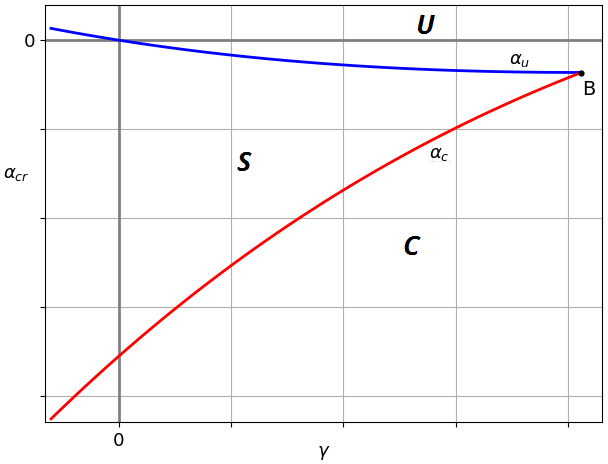
\includegraphics[scale=0.55]{scheme.png}  
\end{figure}

$$ B=(\gamma_*, \alpha_*) $$

\end{frame}

\begin{frame}
\frametitle{ Численные результаты: $ \alpha_c(x_0) $ при $ \gamma = 0 $ }

\begin{figure} 
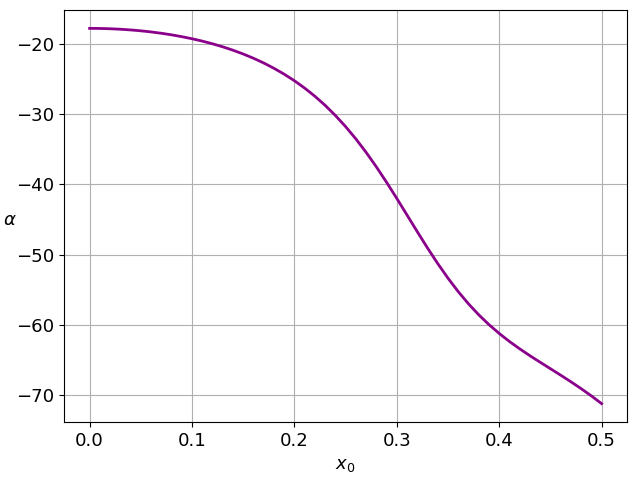
\includegraphics[scale=0.65]{origins.png}  
\end{figure}

\end{frame}

\begin{frame}
\frametitle{ Численные результаты: $ \alpha_{cr}(\gamma) $ }

\begin{figure} 
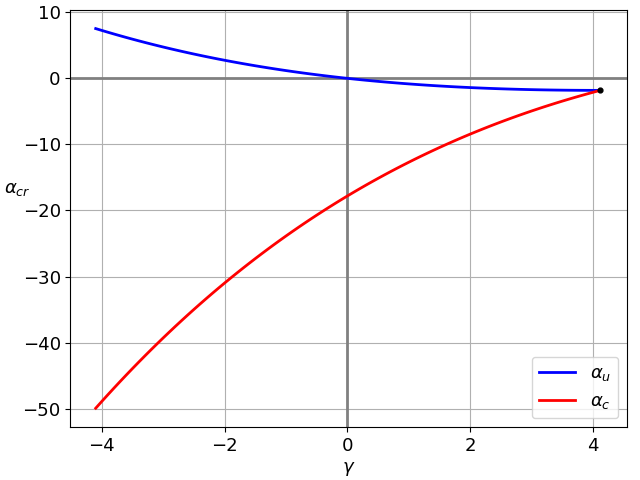
\includegraphics[scale=0.55]{alphas_0.png}  
\end{figure}

$$ x_0 = 0: \quad \gamma_* \approx 4.115 $$

\end{frame}

\begin{frame}
\frametitle{ Численные результаты: $ \alpha_{cr}(\gamma) $ }

\begin{figure} 
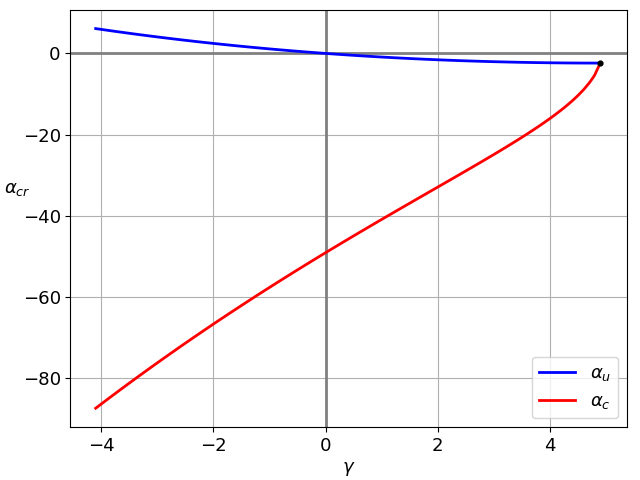
\includegraphics[scale=0.55]{alphas_13.png}  
\end{figure}

$$ x_0 = 0.33: \quad \gamma_* \approx 4.895 $$

\end{frame}

\begin{frame}
\frametitle{ Численные результаты: $ \alpha_{cr}(\gamma) $ }

\begin{figure} 
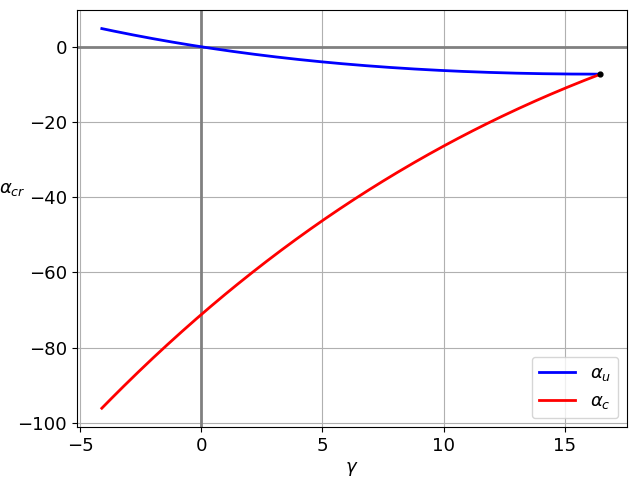
\includegraphics[scale=0.55]{alphas_12.png}  
\end{figure}

$$ x_0 = 0.5: \quad \gamma_* \approx 16.4 $$

\end{frame}

\begin{frame}
\frametitle{ Численные результаты: $ \alpha_{cr}(\gamma) $ }

\begin{figure} 
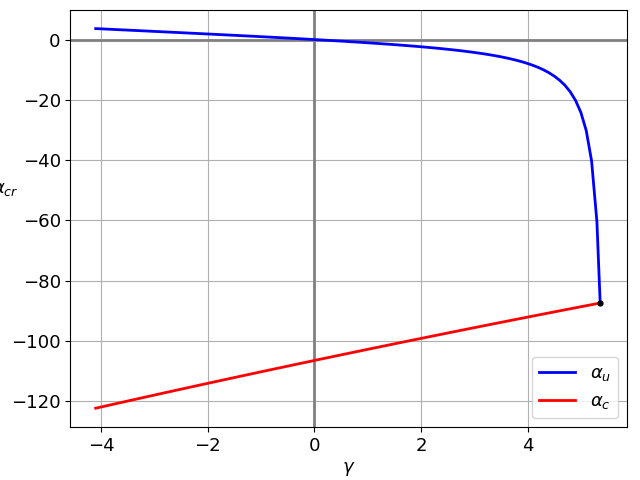
\includegraphics[scale=0.55]{alphas_23.png}  
\end{figure}

$$ x_0 = 0.67: \quad \gamma_* \approx 5.361 $$

\end{frame}

\begin{frame}
\frametitle{ Локальный анализ краевой задачи }

\begin{equation}
	u = \sqrt{\varepsilon}u_0 + \varepsilon u_1 + \varepsilon^{\frac{3}{2}} u_2 + O(\varepsilon^2),
\end{equation}

\bigskip

$$ \varepsilon = | \alpha - \alpha_{cr} |, $$

$$ \varepsilon \ll 1, \quad s = \varepsilon t. $$

\end{frame}

\begin{frame}
\frametitle{ Случай дивергентной потери устойчивости }

\begin{itemize}
\item { $ \lambda = 0: \quad \varepsilon=\alpha-\alpha_u, $
}
\end{itemize}

\medskip

\begin{equation}
	\dot u_0 = u_0'' + \gamma u_0,
\end{equation}
\begin{equation}
	u_0'(0, t) \, = 0, \qquad u_0'(1, t) \, = \alpha_u u_0(x_0, t),
\end{equation}

$$ u_0 = \rho(s) \ch \sqrt{-\gamma} x. $$

\medskip

\begin{equation}
	\dot u_2 + \frac{\partial u_0}{\partial s} = u_2'' + \gamma u_2,
\end{equation}
\begin{equation}
	u_2'(0, t) \, = 0, \qquad u_2'(1, t) \, = \alpha_u u_2(x_0, t) + u_0(x_0, t) + \beta u_0^3(x_0, t),
\end{equation}

\end{frame}

\begin{frame}
\frametitle{ Случай дивергентной потери устойчивости }

$$ u_2 = e^{\lambda t}v_2(x), \quad \lambda = 0, $$

\medskip

\begin{equation}
	v_2'' + \gamma v_2 - \rho' \ch \sqrt{-\gamma} x = 0,
\end{equation}
\begin{equation}
	v_2'(0) \, = 0, \quad v_2'(1) \, = \alpha_u v_2(x_0) + \rho \ch \sqrt{-\gamma} x_0 + \beta \rho^3\ch^3 \sqrt{-\gamma} x_0.
\end{equation}

\medskip

$$ v_2 = c\,\ch \sqrt{-\gamma} x + \frac{\rho'}{2\sqrt{-\gamma}}\sh\sqrt{-\gamma}x + \frac{\rho'x}{2} \ch\sqrt{-\gamma}x, $$
$$ c \in \mathbb{R}. $$

\end{frame}

\begin{frame}
\frametitle{ Случай дивергентной потери устойчивости }

\begin{equation}
	\rho' = \phi_0 \rho + d_0 \rho^3,
\end{equation}

\bigskip

$$ \phi_0 = Q \ch \sqrt{-\gamma} x_0 , $$
$$ d_0 = \beta Q \ch^3 \sqrt{-\gamma} x_0, $$

$$ Q = \frac{2\sqrt{-\gamma}}{\sqrt{-\gamma}\ch\sqrt{-\gamma} + \sh\sqrt{-\gamma} - \alpha_u x_0 \sqrt{-\gamma} x_0}. $$

$$ A = \sqrt{\frac{1}{|\beta| \ch^2 \sqrt{-\gamma} x_0}}. $$

\end{frame}

\begin{frame}
\frametitle{ Численные результаты: $ \phi_0(\gamma) $ и $ d_0(\gamma) $ }

\begin{figure} 
\begin{minipage}[h]{0.49\linewidth}
\begin{center}
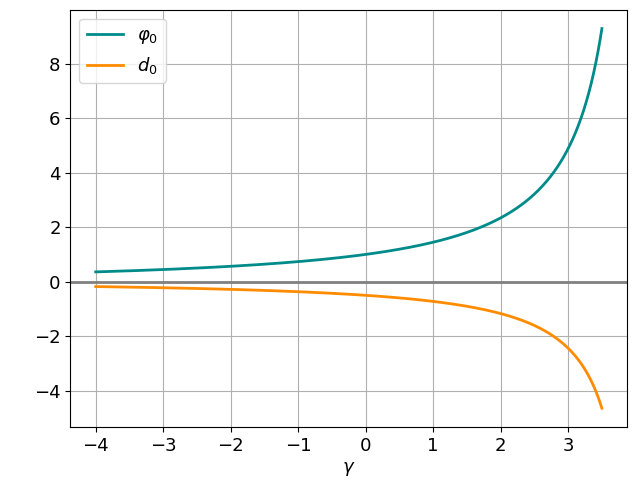
\includegraphics[scale=0.38]{divergent_phi0d0_x0=0,0,beta=-0,5.png} \\ {\scriptsize a) $ \beta = -0.5 $}
\end{center}
\end{minipage} 
\hfill
\begin{minipage}[h]{0.49\linewidth}
\begin{center}
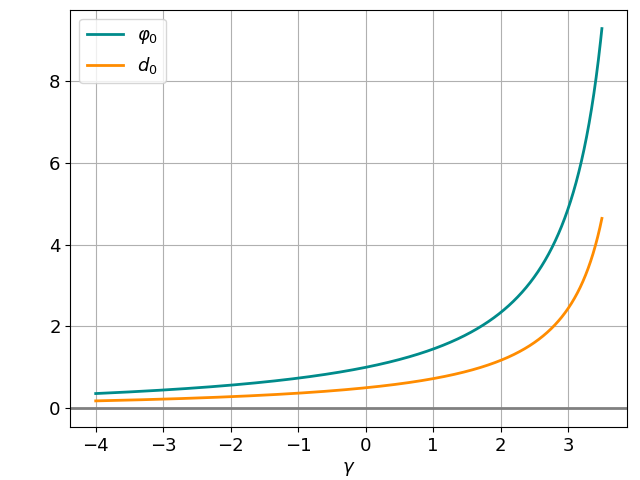
\includegraphics[scale=0.38]{divergent_phi0d0_x0=0,0,beta=0,5.png}  \\ {\scriptsize b) $ \beta = 0.5 $}
\end{center}
\end{minipage} 
\end{figure}

$$ x_0 = 0.0 $$

\end{frame}

\begin{frame}
\frametitle{ Численные результаты: $ \phi_0(\gamma) $ и $ d_0(\gamma) $ }

\begin{figure} 
\begin{minipage}[h]{0.49\linewidth}
\begin{center}
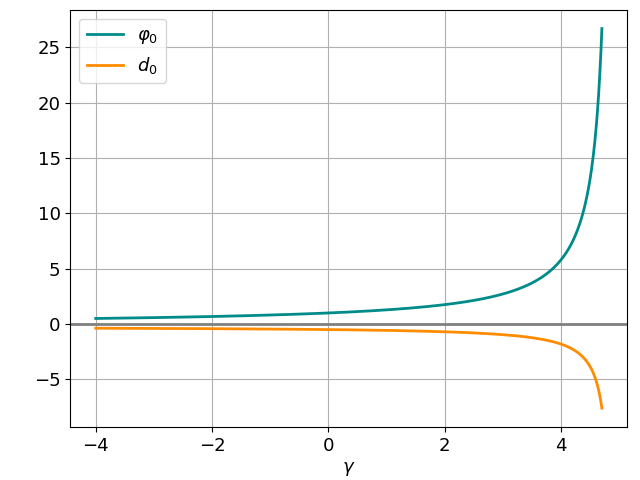
\includegraphics[scale=0.38]{divergent_phi0d0_x0=0,33,beta=-0,5.png} \\ {\scriptsize a) $ \beta = -0.5 $}
\end{center}
\end{minipage} 
\hfill
\begin{minipage}[h]{0.49\linewidth}
\begin{center}
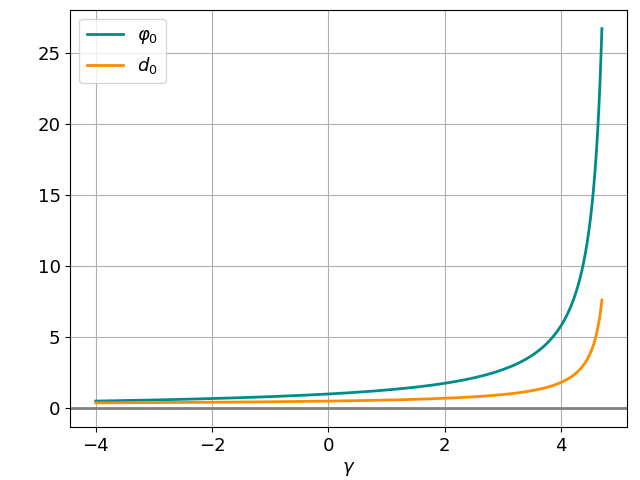
\includegraphics[scale=0.38]{divergent_phi0d0_x0=0,33,beta=0,5.png}  \\ {\scriptsize b) $ \beta = 0.5 $}
\end{center}
\end{minipage} 
\end{figure}

$$ x_0 = 0.33 $$

\end{frame}

\begin{frame}
\frametitle{ Численные результаты: $ \phi_0(\gamma) $ и $ d_0(\gamma) $ }

\begin{figure} 
\begin{minipage}[h]{0.49\linewidth}
\begin{center}
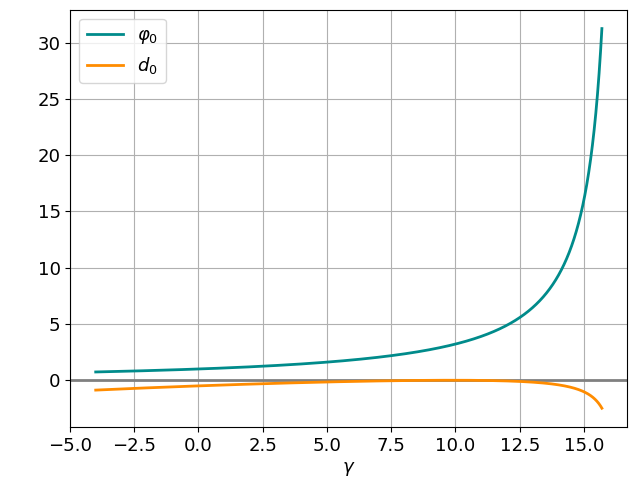
\includegraphics[scale=0.38]{divergent_phi0d0_x0=0,5,beta=-0,5.png} \\ {\scriptsize a) $ \beta = -0.5 $}
\end{center}
\end{minipage} 
\hfill
\begin{minipage}[h]{0.49\linewidth}
\begin{center}
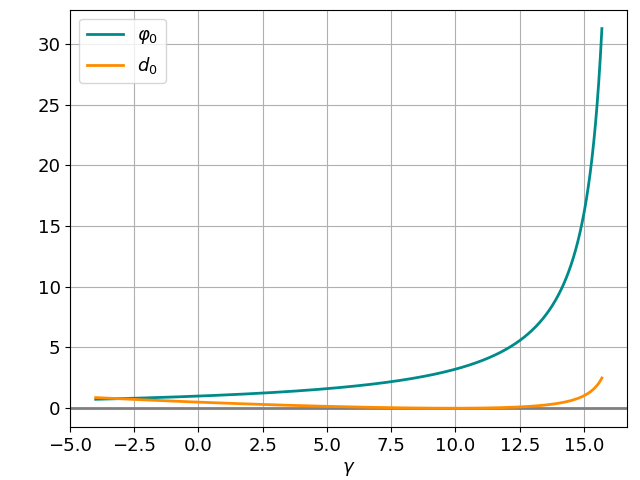
\includegraphics[scale=0.38]{divergent_phi0d0_x0=0,5,beta=0,5.png}  \\ {\scriptsize b) $ \beta = 0.5 $}
\end{center}
\end{minipage} 
\end{figure}

$$ x_0 = 0.5 $$

\end{frame}

\begin{frame}
\frametitle{ Численные результаты: $ \phi_0(\gamma) $ и $ d_0(\gamma) $ }

\begin{figure} 
\begin{minipage}[h]{0.49\linewidth}
\begin{center}
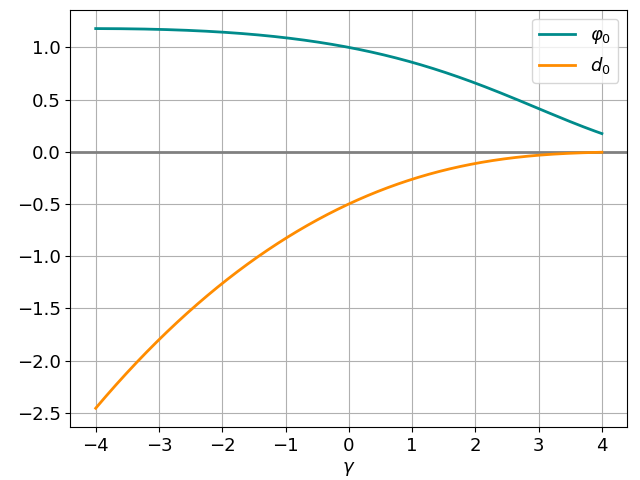
\includegraphics[scale=0.38]{divergent_phi0d0_x0=0,67,beta=-0,5.png} \\ {\scriptsize a) $ \beta = -0.5 $}
\end{center}
\end{minipage} 
\hfill
\begin{minipage}[h]{0.49\linewidth}
\begin{center}
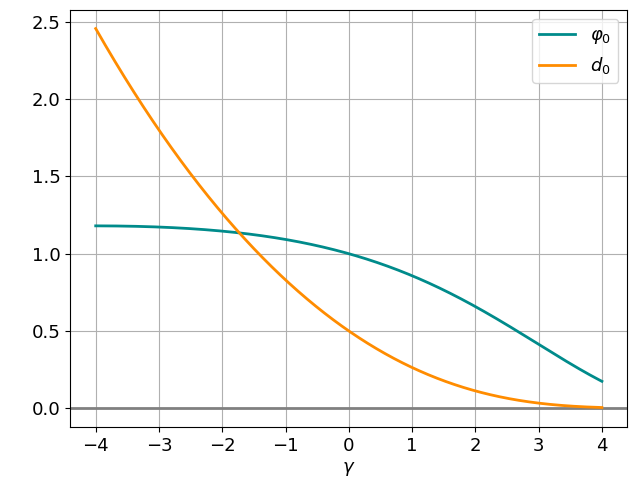
\includegraphics[scale=0.38]{divergent_phi0d0_x0=0,67,beta=0,5.png}  \\ {\scriptsize b) $ \beta = 0.5 $}
\end{center}
\end{minipage} 
\end{figure}

$$ x_0 = 0.67 $$

\end{frame}

\begin{frame}
\frametitle{ Численные результаты: $ \phi_0(\gamma) $ и $ d_0(\gamma) $ для $ x_0 \in \left( \frac{1}{3}, \frac{1}{2} \right) $ }

\begin{figure} 
\begin{minipage}[h]{0.49\linewidth}
\begin{center}
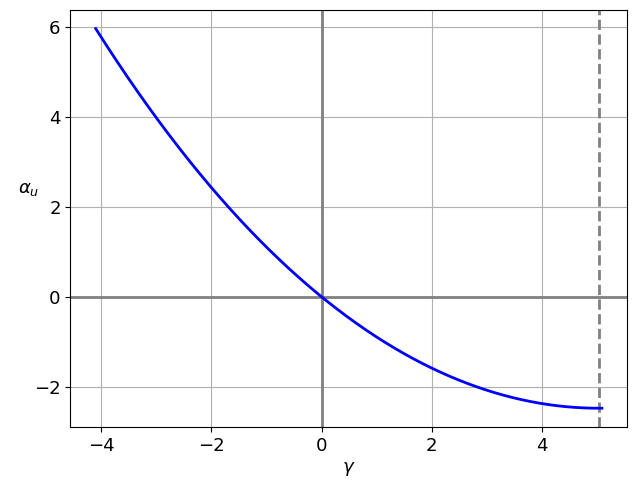
\includegraphics[scale=0.38]{x0=0,35.png} \\ {\scriptsize a) $ \widetilde{\gamma} \approx 5.0 $}
\end{center}
\end{minipage} 
\hfill
\begin{minipage}[h]{0.49\linewidth}
\begin{center}
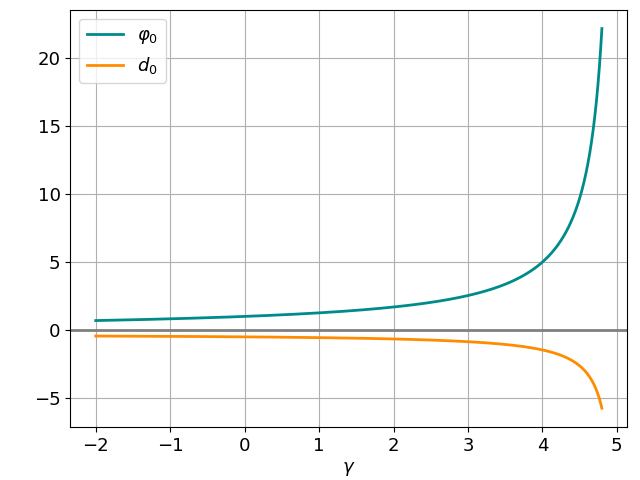
\includegraphics[scale=0.38]{divergent_phi0d0_x0=0,35,beta=-0,5_before.png}  \\ {\scriptsize b) $ \gamma <  \widetilde{\gamma}, \; \beta = -0.5 $}
\end{center}
\end{minipage} 
\end{figure}

$$ x_0 = 0.35 $$

\end{frame}


\begin{frame}
\frametitle{ Численные результаты: $ \phi_0(\gamma) $ и $ d_0(\gamma) $ для $ x_0 \in \left( \frac{1}{3}, \frac{1}{2} \right) $ }

\begin{figure} 
\begin{minipage}[h]{0.49\linewidth}
\begin{center}
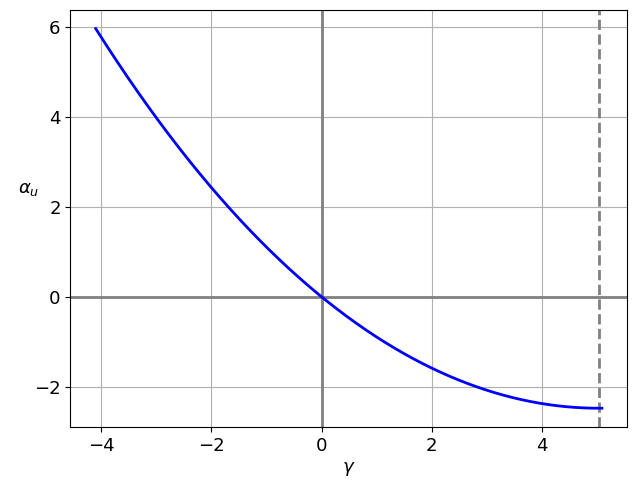
\includegraphics[scale=0.38]{x0=0,35.png} \\ {\scriptsize a) $ \widetilde{\gamma} \approx 5.0 $}
\end{center}
\end{minipage} 
\hfill
\begin{minipage}[h]{0.49\linewidth}
\begin{center}
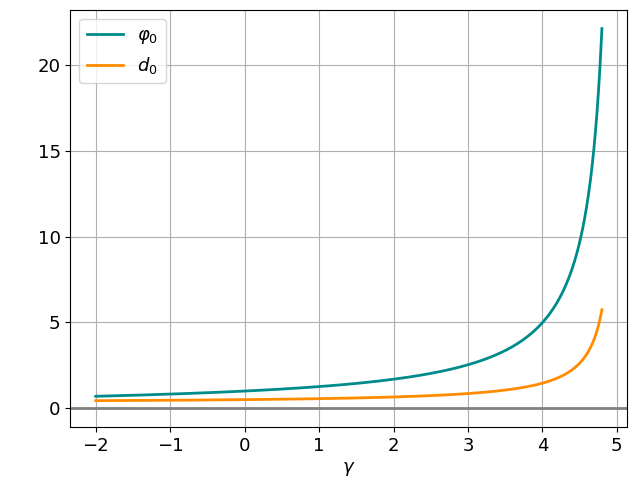
\includegraphics[scale=0.38]{divergent_phi0d0_x0=0,35,beta=0,5_before.png}  \\ {\scriptsize b) $ \beta = -0.5 $}
\end{center}
\end{minipage} 
\end{figure}

$$ x_0 = 0.35 $$

\end{frame}

\begin{frame}
\frametitle{ Численные результаты: $ \phi_0(\gamma) $ и $ d_0(\gamma) $ для $ x_0 \in \left( \frac{1}{3}, \frac{1}{2} \right) $ }

\begin{figure} 
\begin{minipage}[h]{0.49\linewidth}
\begin{center}
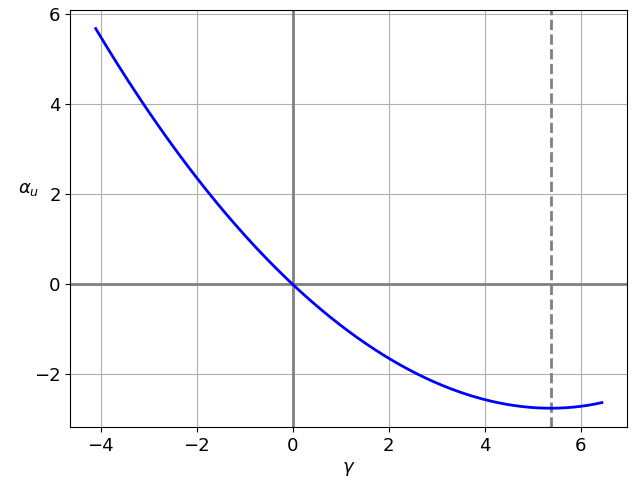
\includegraphics[scale=0.38]{x0=0,39.png} \\ {\scriptsize a) $ \widetilde{\gamma} \approx 5.37 $}
\end{center}
\end{minipage} 
\hfill
\begin{minipage}[h]{0.49\linewidth}
\begin{center}
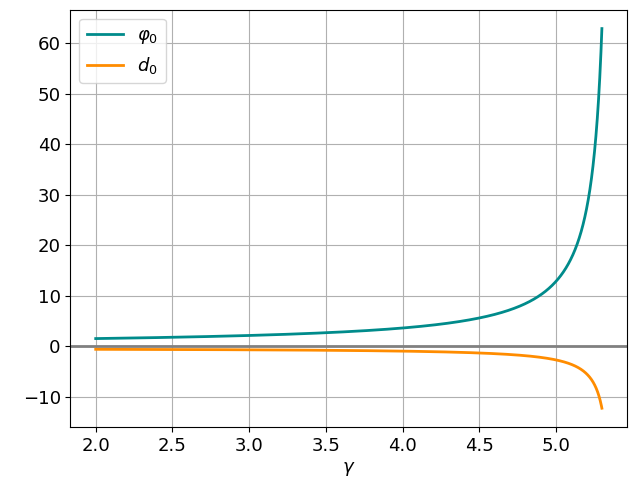
\includegraphics[scale=0.38]{divergent_phi0d0_x0=0,39,beta=-0,5_before.png}  \\ {\scriptsize b) $ \beta = -0.5 $}
\end{center}
\end{minipage} 
\end{figure}

$$ x_0 = 0.39 $$

\end{frame}

\begin{frame}
\frametitle{ Численные результаты: $ \phi_0(\gamma) $ и $ d_0(\gamma) $ для $ x_0 \in \left( \frac{1}{3}, \frac{1}{2} \right) $ }

\begin{figure} 
\begin{minipage}[h]{0.49\linewidth}
\begin{center}
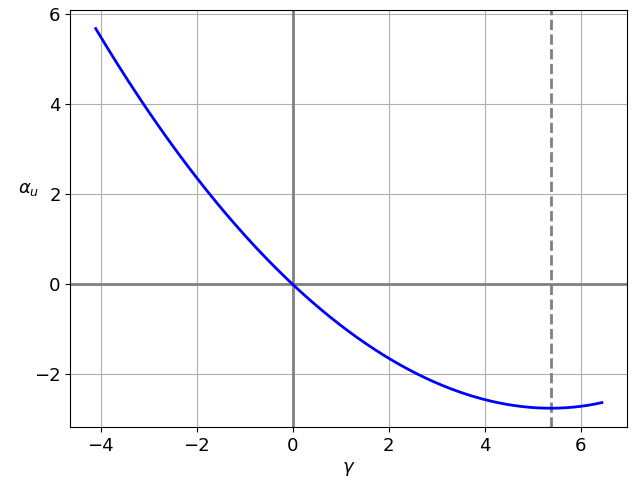
\includegraphics[scale=0.38]{x0=0,39.png} \\ {\scriptsize a) $ \widetilde{\gamma} \approx 5.37 $}
\end{center}
\end{minipage} 
\hfill
\begin{minipage}[h]{0.49\linewidth}
\begin{center}
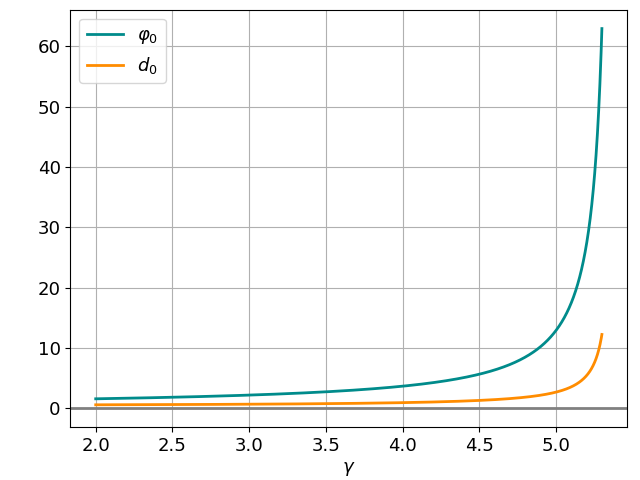
\includegraphics[scale=0.38]{divergent_phi0d0_x0=0,39,beta=0,5_before.png}  \\ {\scriptsize b) $ \beta = -0.5 $}
\end{center}
\end{minipage} 
\end{figure}

$$ x_0 = 0.39 $$

\end{frame}

\begin{frame}
\frametitle{ Численные результаты: $ \phi_0(\gamma) $ и $ d_0(\gamma) $ для $ x_0 \in \left( \frac{1}{3}, \frac{1}{2} \right) $ }

\begin{figure} 
\begin{minipage}[h]{0.49\linewidth}
\begin{center}
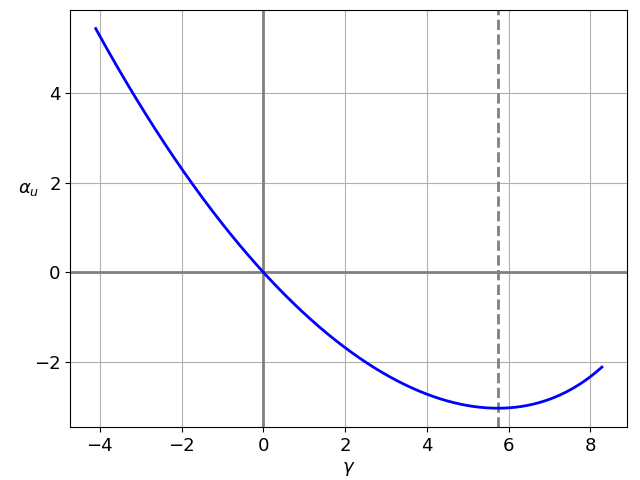
\includegraphics[scale=0.38]{x0=0,42.png} \\ {\scriptsize a) $ \widetilde{\gamma} \approx 5.73 $}
\end{center}
\end{minipage} 
\hfill
\begin{minipage}[h]{0.49\linewidth}
\begin{center}
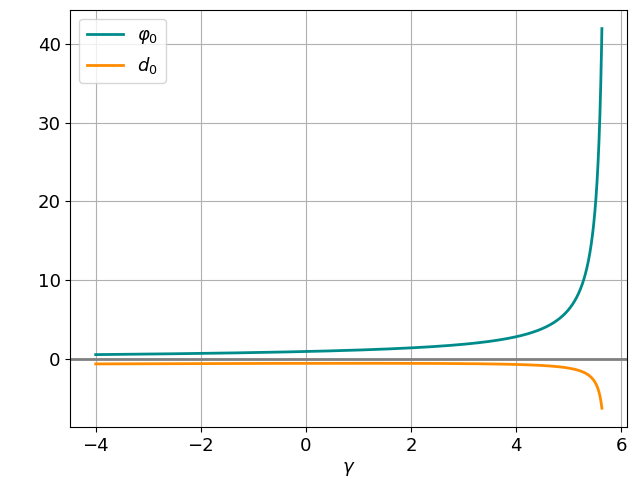
\includegraphics[scale=0.38]{divergent_phi0d0_x0=0,42,beta=-0,5_before.png}  \\ {\scriptsize b) $ \beta = -0.5 $}
\end{center}
\end{minipage} 
\end{figure}

$$ x_0 = 0.42 $$

\end{frame}

\begin{frame}
\frametitle{ Численные результаты: $ \phi_0(\gamma) $ и $ d_0(\gamma) $ для $ x_0 \in \left( \frac{1}{3}, \frac{1}{2} \right) $ }

\begin{figure} 
\begin{minipage}[h]{0.49\linewidth}
\begin{center}
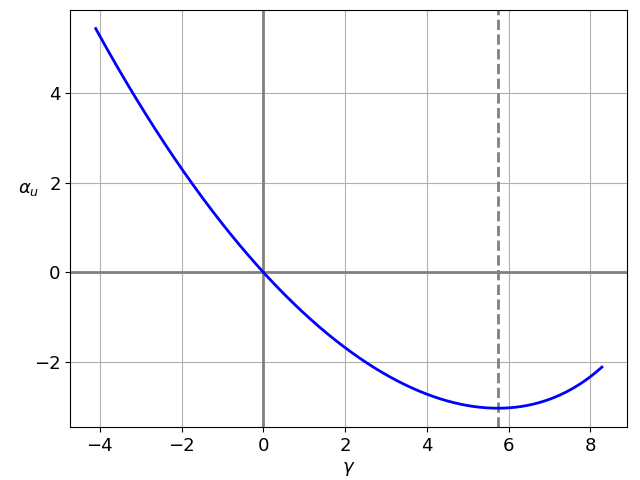
\includegraphics[scale=0.38]{x0=0,42.png} \\ {\scriptsize a) $ \widetilde{\gamma} \approx 5.73 $}
\end{center}
\end{minipage} 
\hfill
\begin{minipage}[h]{0.49\linewidth}
\begin{center}
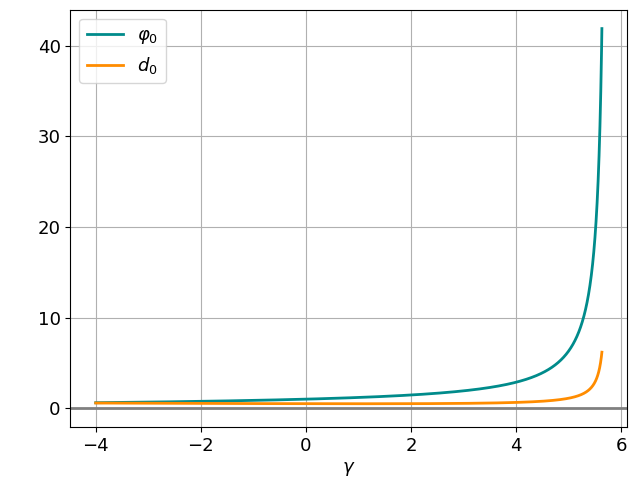
\includegraphics[scale=0.38]{divergent_phi0d0_x0=0,42,beta=0,5_before.png}  \\ {\scriptsize b) $ \beta = -0.5 $}
\end{center}
\end{minipage} 
\end{figure}

$$ x_0 = 0.42 $$

\end{frame}

\begin{frame}
\frametitle{ Численные результаты: $ \phi_0(\gamma) $ и $ d_0(\gamma) $ для $ x_0 \in \left( \frac{1}{3}, \frac{1}{2} \right) $ }

\begin{figure} 
\begin{minipage}[h]{0.49\linewidth}
\begin{center}
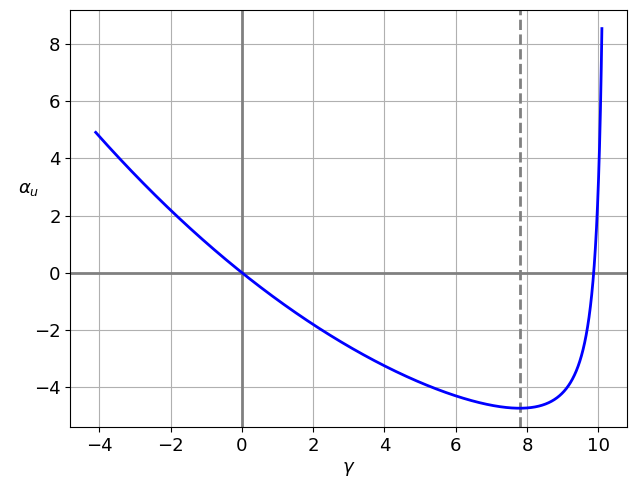
\includegraphics[scale=0.38]{x0=0,49.png} \\ {\scriptsize a) $ \widetilde{\gamma} \approx 7.79 $}
\end{center}
\end{minipage} 
\hfill
\begin{minipage}[h]{0.49\linewidth}
\begin{center}
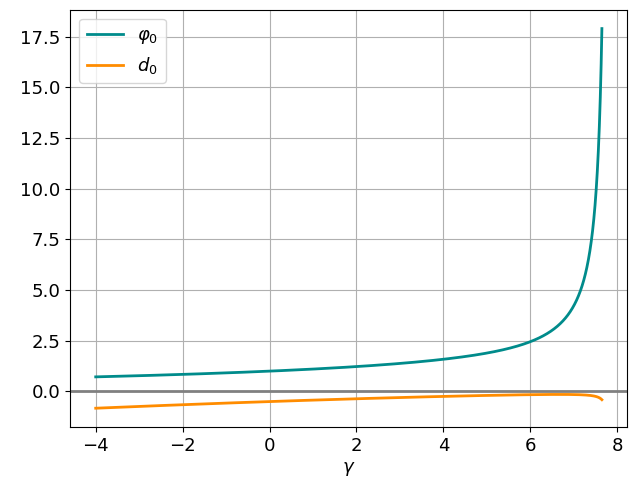
\includegraphics[scale=0.38]{divergent_phi0d0_x0=0,49,beta=-0,5_before.png}  \\ {\scriptsize b) $ \beta = -0.5 $}
\end{center}
\end{minipage} 
\end{figure}

$$ x_0 = 0.49 $$

\end{frame}

\begin{frame}
\frametitle{ Численные результаты: $ \phi_0(\gamma) $ и $ d_0(\gamma) $ для $ x_0 \in \left( \frac{1}{3}, \frac{1}{2} \right) $ }

\begin{figure} 
\begin{minipage}[h]{0.49\linewidth}
\begin{center}
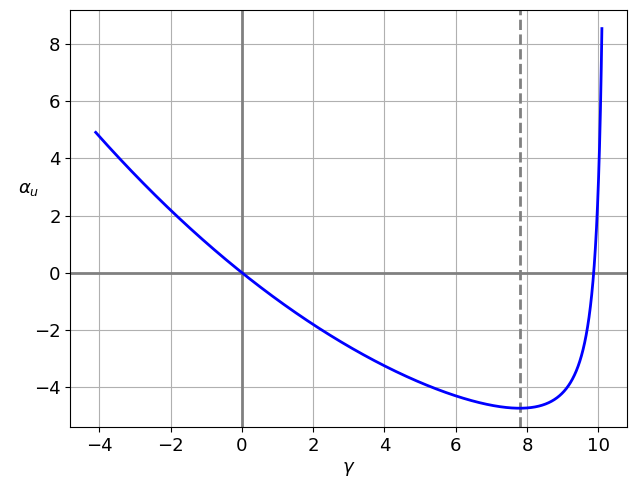
\includegraphics[scale=0.38]{x0=0,49.png} \\ {\scriptsize a) $ \widetilde{\gamma} \approx 7.79 $}
\end{center}
\end{minipage} 
\hfill
\begin{minipage}[h]{0.49\linewidth}
\begin{center}
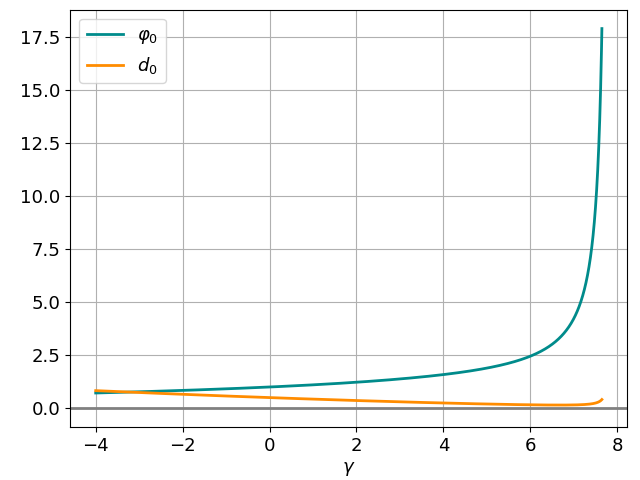
\includegraphics[scale=0.38]{divergent_phi0d0_x0=0,49,beta=0,5_before.png}  \\ {\scriptsize b) $ \beta = -0.5 $}
\end{center}
\end{minipage} 
\end{figure}

$$ x_0 = 0.49 $$

\end{frame}

\begin{frame}
\frametitle{ Случай дивергентной потери устойчивости }

\begin{rustheorem}
В краевой задаче (1), (2) для собственного значения $ \lambda = 0 $ и $ \alpha = \alpha_u + \varepsilon $, где $ \alpha_u $ вычисляется по формуле (8), а $ \varepsilon \ll 1 $, $ \forall \beta > 0 $ имеет место быть грубая потеря устойчивости нулевого состояния равновесия. При этом $ \forall \beta < 0 $ и $ \gamma < \widetilde{\gamma} $, где 
\begin{equation*}
    \begin{matrix}
    \widetilde{\gamma} =
    & \left\{
    \begin{matrix}
        \gamma_0: \; F(\gamma_0, \alpha, x_0) = 0, & \mbox{если } x_0 \in \left( \frac{1}{3}, \frac{1}{2} \right), \\
        \gamma_*, & \mbox{иначе, }, \\
    \end{matrix} \right.
    \end{matrix}
\end{equation*}
а $ F(\gamma, \alpha, x_0) = \alpha\,x_0\sh\sqrt{-\gamma}x_0 - \sh\sqrt{-\gamma} - \sqrt{-\gamma} \ch\sqrt{-\gamma}  $, нулевое решение краевой задачи (1), (2) дивергентно теряет свою устойчивость.
\end{rustheorem}

\end{frame}

\begin{frame}
\frametitle{ Случай колебательной потери устойчивости }

\begin{itemize}
\item { $ \lambda = \pm i \omega: \quad \varepsilon=\alpha_c-\alpha, $
}
\end{itemize}

\medskip

\begin{equation}
	\dot u_0 = u_0'' + \gamma u_0,
\end{equation}
\begin{equation}
	u_0'(0, t) \, = 0, \qquad u_0'(1, t) \, = \alpha_c u_0(x_0, t),
\end{equation}

$$ u_0 = z(s) e^{i \omega t} \ch \mu x + \overline{z(s)} e^{-i \omega t} \overline{\ch \mu x}, $$

$$ \mu = \sqrt{-\gamma+i \omega}. $$

\medskip

\begin{equation}
	\dot u_2 + \frac{\partial u_0}{\partial s} = u_2'' + \gamma u_2,
\end{equation}
\begin{equation}
	u_2'(0, t) \, = 0, \qquad u_2'(1, t) \, = \alpha_c u_2(x_0, t) - u_0(x_0, t) + \beta u_0^3(x_0, t),
\end{equation}

\end{frame}

\begin{frame}
\frametitle{ Случай колебательной потери устойчивости }

$$ u_2 = e^{i \omega t} v_2(x), $$

\bigskip

\begin{equation}
	v_2'' + (\gamma - i \omega) v_2 - z' w(x) = 0,
\end{equation}
\begin{equation}
	v_2'(0) \, = 0, \qquad v_2'(1) \, = \alpha_u v_2(x_0) - z w(x_0) + 3\beta z|z|^2 w|w|^2,
\end{equation}

$$ w(x) = \ch \mu x. $$

\end{frame}

\begin{frame}
\frametitle{ Случай колебательной потери устойчивости }

\begin{equation}
	z' = \phi z + d z |z|^2,
\end{equation}

$$ \phi_0 = \mbox{Re} \phi, \quad d_0 = \mbox{Re} d, $$

\bigskip

$$ \phi = -2Q\ch \mu x_0, $$

$$ d = 1.5 \beta Q ( \ch(\mu + 2\,\mbox{Re}\mu)x_0 + \ch(\mu + 2i\,\mbox{Im}\mu)x_0 + 2\ch\overline{\mu}x_0 ), $$

$$ \mu = \sqrt{-\gamma + i \omega}, $$ 
$$ Q = \frac{\mu}{\mu \ch \mu + \sh \mu - \alpha_c x_0 \sh \mu x_0} $$

\end{frame}

\begin{frame}
\frametitle{ Численные результаты: $ \phi_0(\gamma) $ и $ d_0(\gamma) $ }

\begin{figure} 
\begin{minipage}[h]{0.49\linewidth}
\begin{center}
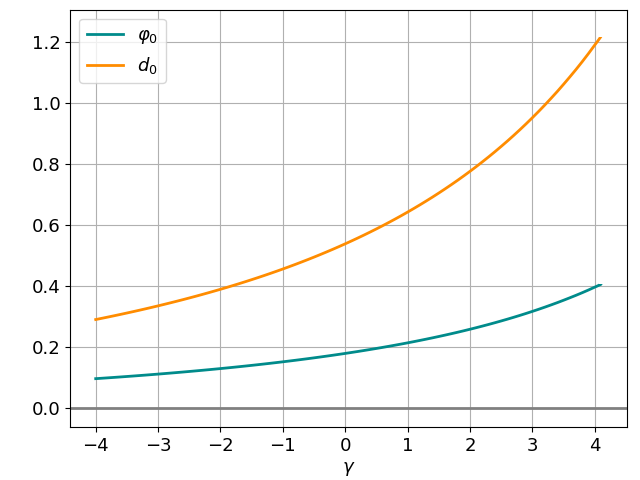
\includegraphics[scale=0.35]{oscillating_phi0d0_x0=0,0,beta=-1,0.png} \\ {\scriptsize a) $ \beta = -1.0 $}
\end{center}
\end{minipage} 
\hfill
\begin{minipage}[h]{0.49\linewidth}
\begin{center}
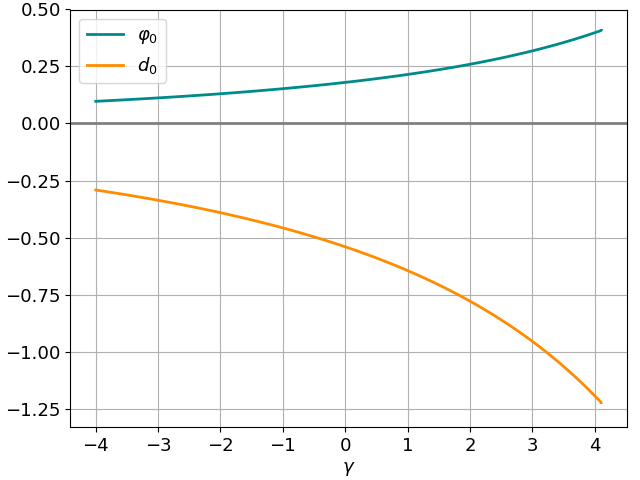
\includegraphics[scale=0.35]{oscillating_phi0d0_x0=0,0_beta=1,0.png}  \\ {\scriptsize b) $ \beta = 1.0 $}
\end{center}
\end{minipage} 
\end{figure}

$$ x_0 = 0.0 $$

\end{frame}

\begin{frame}
\frametitle{ Численные результаты: $ \phi_0(\gamma) $ и $ d_0(\gamma) $ }

\begin{figure} 
\begin{minipage}[h]{0.49\linewidth}
\begin{center}
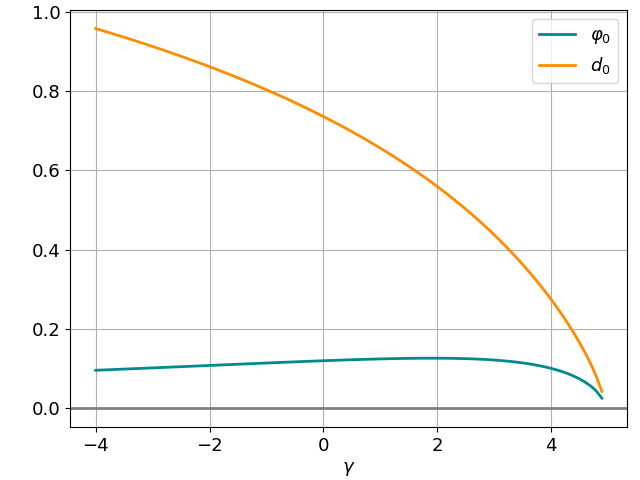
\includegraphics[scale=0.35]{oscillating_phi0d0_x0=0,33,beta=-1,0.png} \\ {\scriptsize a) $ \beta = -1.0 $}
\end{center}
\end{minipage} 
\hfill
\begin{minipage}[h]{0.49\linewidth}
\begin{center}
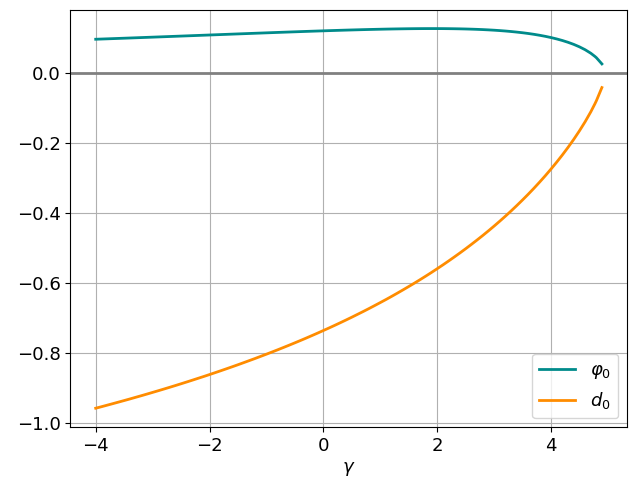
\includegraphics[scale=0.35]{oscillating_phi0d0_x0=0,33,beta=1,0.png}  \\ {\scriptsize b) $ \beta = 1.0 $}
\end{center}
\end{minipage} 
\end{figure}

$$ x_0 = 0.33 $$

\end{frame}

\begin{frame}
\frametitle{ Численные результаты: $ \alpha_c(x_0) $ при $ \gamma = 0 $ }

\begin{figure} 
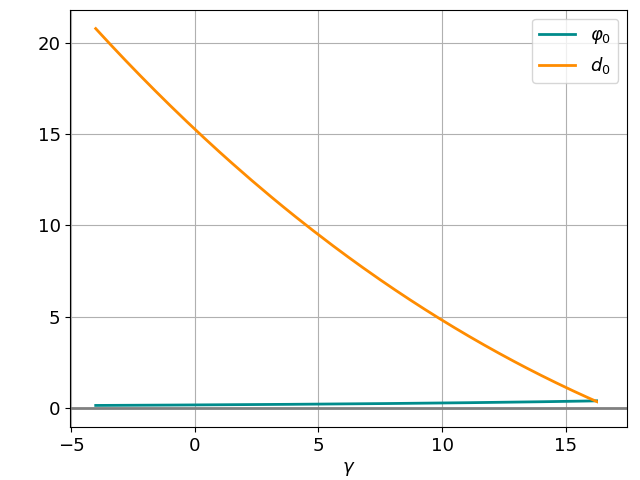
\includegraphics[scale=0.5]{oscillating_phi0d0_x0=0,5,beta=-1,0.png}  
\end{figure}

$$ x_0 = 0.5, \quad \beta=-1.0 $$

\end{frame}

\begin{frame}
\frametitle{ Численные результаты: $ \phi_0(\gamma) $ и $ d_0(\gamma) $ }

\begin{figure} 
\begin{minipage}[h]{0.49\linewidth}
\begin{center}
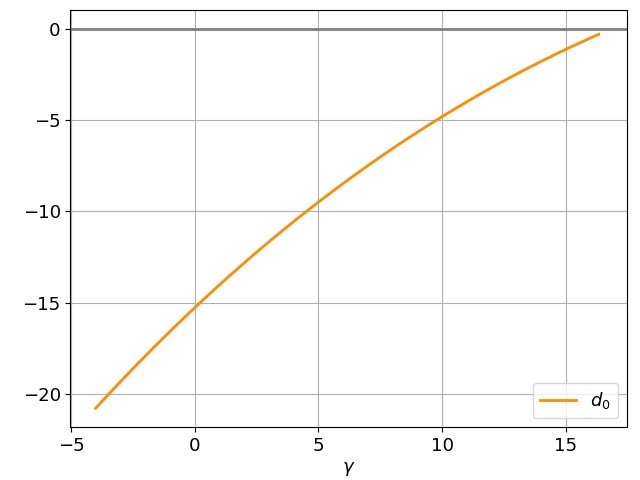
\includegraphics[scale=0.35]{oscillating_d0_x0=0,5,beta=1,0.png}
\end{center}
\end{minipage} 
\hfill
\begin{minipage}[h]{0.49\linewidth}
\begin{center}
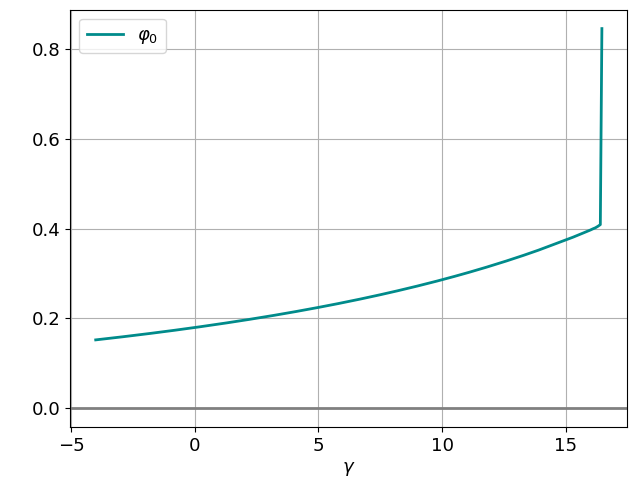
\includegraphics[scale=0.35]{oscillating_phi0_x0=0,5,beta=1,0.png}
\end{center}
\end{minipage} 
\end{figure}

$$ x_0 = 0.5, \quad \beta=1.0 $$

\end{frame}

\begin{frame}
\frametitle{ Численные результаты: $ \phi_0(\gamma) $ и $ d_0(\gamma) $ }

\begin{figure} 
\begin{minipage}[h]{0.49\linewidth}
\begin{center}
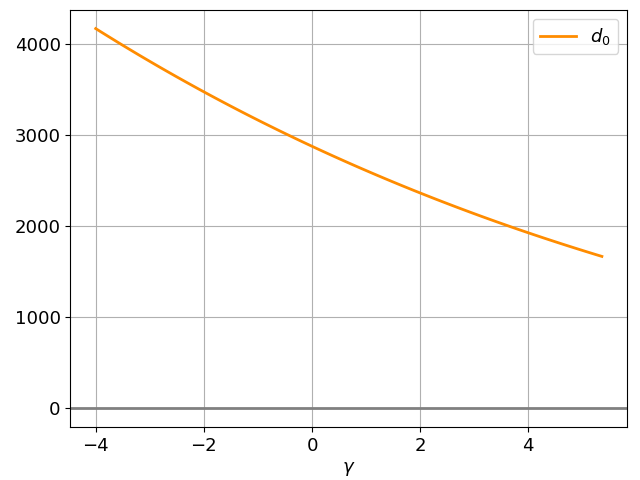
\includegraphics[scale=0.35]{oscillating_d0_x0=0,67,beta=-1,0.png}
\end{center}
\end{minipage} 
\hfill
\begin{minipage}[h]{0.49\linewidth}
\begin{center}
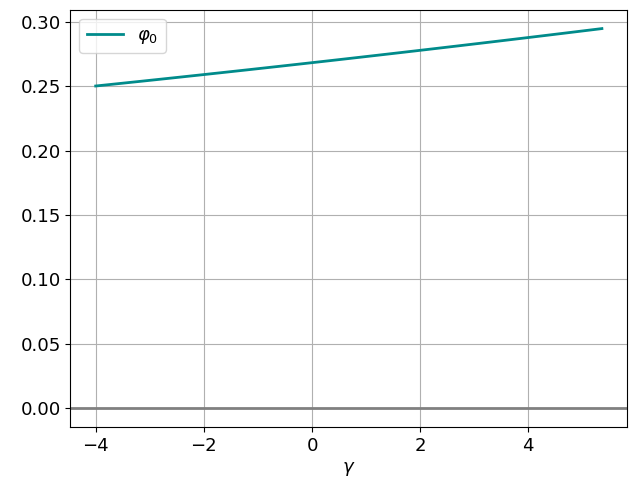
\includegraphics[scale=0.35]{oscillating_phi0_x0=0,67,beta=-1,0.png}
\end{center}
\end{minipage} 
\end{figure}

$$ x_0 = 0.67, \quad \beta=-1.0 $$

\end{frame}

\begin{frame}
\frametitle{ Численные результаты: $ \phi_0(\gamma) $ и $ d_0(\gamma) $ }

\begin{figure} 
\begin{minipage}[h]{0.49\linewidth}
\begin{center}
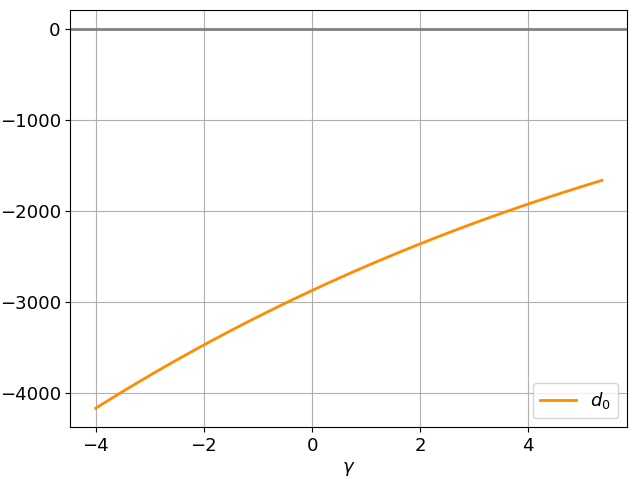
\includegraphics[scale=0.35]{oscillating_d0_x0=0,67,beta=1,0.png}
\end{center}
\end{minipage} 
\hfill
\begin{minipage}[h]{0.49\linewidth}
\begin{center}
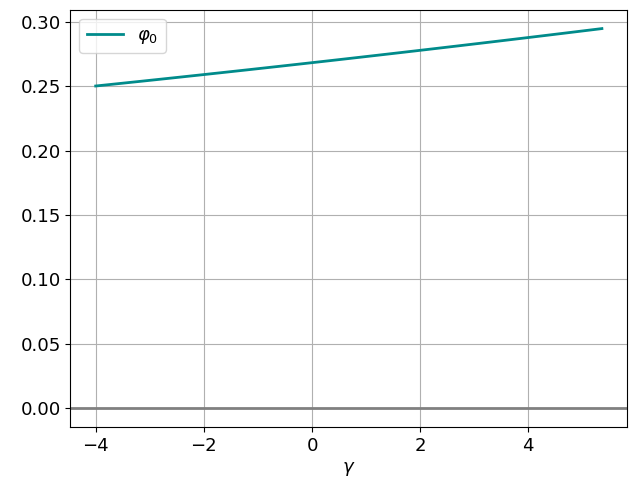
\includegraphics[scale=0.35]{oscillating_phi0_x0=0,67,beta=1,0.png}
\end{center}
\end{minipage} 
\end{figure}

$$ x_0 = 0.67, \quad \beta=1.0 $$

\end{frame}

\begin{frame}
\frametitle{ Случай колебательной потери устойчивости }

\begin{rustheorem}
В краевой задаче (1), (2) для собственного значения $ \lambda = \pm i \omega $ и $ \alpha = \alpha_c - \varepsilon $, где $ \alpha_c $ вычисляется по формуле (9), а $ \varepsilon \ll 1 $, $ \forall \beta < 0 $ имеет место быть грубая потеря устойчивости нулевого состояния равновесия. При этом $ \forall \beta > 0 $ нулевое решение краевой задачи (1), (2) колебательно теряет свою устойчивость.
\end{rustheorem}

\end{frame}

\end{document}